\pagestyle{empty}

\begin{tcbposter}[
  coverage = {
      spread,
      %interior style={bottom color=white},
      watermark text={BIND},
      watermark color=black!25!white,
      watermark opacity=0.4
  },
  poster   = {showframe=false,columns=30,rows=12},
  boxes    = {
      enhanced standard jigsaw,sharp corners=downhill,arc=7mm,boxrule=.6mm,
      colback=white,opacityback=0.7,colframe=black,
      title style={left color=black,right color=white},
      fonttitle=\bfseries
   }
]

%----
% try removing 'interior engine'
\posterbox[blankest,interior engine=path, halign=center,valign=center,colupper=white!25!black,
	]{name=title,column=1,span=29,below=top}{
		\vspace{.3cm}
		\begin{tabular}{llllll}
			Name: & \vlongline & Player: & \vlongline & Code: & \vlongline \\
			\\
			Concept: & \vlongline & Race: & \vlongline & Culture: & \vlongline \\
		\end{tabular}
		\vspace{0.3cm}
}

%----
	\posterbox[adjusted title=Attributes (5 \textbar~10/20/30/50)]{name=attributes,column=1,row=2,span=10,rowspan=2}{\vspace{-.3cm}\begin{tabular}{ll}
		& {\tiny Penalties \hspace{30pt} Bonuses} \\
		Strength & \attributecircles \\
		Dexterity & \attributecircles \\
		Speed & \attributecircles \\
		Intelligence & \attributecircles \\
		Wits & \attributecircles \\
		Charisma & \attributecircles \\
	\end{tabular}}
%----

	\posterbox{name=gumption,column=11,row=2,span=8,rowspan=2}{

	\vspace{.2cm} {\small HP \tiny{(6 + Str)}}

	\begin{tabular}{p{0em}p{0em}p{0em}p{0em}p{0em}p{0em}p{0em}p{0em}p{0em}p{0em}}

		\ding{108} & \ding{109} & \ding{109} & \ding{109} & \ding{109} & \ding{109} & \ding{109} & \ding{109} & \ding{109} & \ding{109}  \\
		\tenboxes
	\end{tabular}

	\vspace{.6cm} {\small Fatigue}

	\begin{tabular}{p{0em}p{0em}p{0em}p{0em}p{0em}p{0em}p{0em}p{0em}p{0em}p{0em}}

	\tenboxes
		\ding{111} & \ding{111} & \ding{111} & \ding{111} & \ding{111} \\
		\ding{182} & \ding{183} & \ding{184} & \ding{185} & \ding{186} & \\
	\end{tabular}

	}
%----
	\posterbox{name=mp,column=19,row=2,span=8,rowspan=2}{

		\vspace{.2cm} {\small FP (10/15/20)} \shortline {\tiny $+ Cha$}

	\begin{tabular}{p{0em}p{0em}p{0em}p{0em}p{0em}p{0em}p{0em}p{0em}p{0em}p{0em}}

		\tencircles
		\tenboxes
		\tencircles
		\tenboxes
	\end{tabular}

		\vspace{.2cm} {\small MP} {\tiny $=2\times spheres +Int$}

	\begin{tabular}{p{0em}p{0em}p{0em}p{0em}p{0em}p{0em}p{0em}p{0em}p{0em}}

	\ding{109} & \ding{109} & \ding{109} & \ding{109} & \ding{109} & \ding{109} & \ding{109} & \ding{109} & \ding{109}  \\
		\ding{111} & \ding{111} & \ding{111} & \ding{111} & \ding{111} & \ding{111} & \ding{111} & \ding{111} & \ding{111}  \\
	\end{tabular}



		}

%----

		\setcounter{track}{18}
		\posterbox{name=track,column=27,row=1,span=3,rowspan=11.8}{ 
			{\large

			\Repeat{18}{\tracker}


			}

			}

%----

		\posterbox[adjusted title=Damage]{name=track,column=1,row=4,span=4,rowspan=1}{ 
	\tiny{(Strength)}
}

%----

	\posterbox[blankest]{name=factors,column=3,row=4}{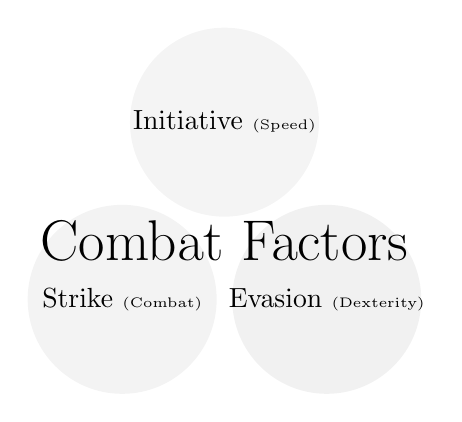
\begin{tikzpicture}
  \begin{scope}[blend group = soft light]
    \fill[gray!11!white,opacity=0.8]   ( 90:1.5) circle (1.2);
    \fill[gray!12!white,opacity=0.8] (210:1.5) circle (1.2);
    \fill[gray!13!white,opacity=0.8]  (330:1.5) circle (1.2);
  \end{scope}
  \node at ( 90:1.5)    {Initiative \tiny{(Speed)}};
  \node at ( 210:1.5)   {Strike \tiny{(Combat)}};
  \node at ( 330:1.5)   {Evasion \tiny{(Dexterity)}};
  \node [font=\huge] {Combat Factors};
\end{tikzpicture}}

%----

	\posterbox{name=initbox,column=1,row=7,span=8,rowspan=1.1}{\begin{multicols}{2}{\tiny \begin{tabular}{lc}
		{\bf Action} & {\bf Cost} \\\hline
		Draw Weapon & 2 \\
		Guarding & 2 \\
		Ram & 3 \\
		Light Weapon & 4 \\
		Med. Weapon & 6 \\
		Use Item & 8 \\
		Spell & 3+lv. \\
		
	\end{tabular}}
		{\tiny \begin{tabular}{lc}
		{\textbf Quick Actions} & \\\hline
		Charge & 0 \\
		Evasion & 2 \\
		Keep Edgy & 2 \\
		Move & 2 \\
		Speak & 2 \\
		\end{tabular}}

	\end{multicols}
}
%----

	\posterbox[adjusted title=Racial Abilities]{name=racial_abilities,column=12,row=7,rowspan=1,span=15}{}

%----
	\posterbox[adjusted title=Armoury]{name=armoury,column=12,row=4,span=15,rowspan=3}{
		\begin{tabular}{p{.2\textwidth}lllll}
			Weapon & Dam. & Init. & Ev. & Wt. & Knack \\
			\\
			
			\writeline & \shortline & \shortline & \shortline &\shortline &  \writeline \\
			\writeline & \shortline & \shortline & \shortline &\shortline &  \writeline \\
			\writeline & \shortline & \shortline & \shortline &\shortline &  \writeline \\
			\writeline & \shortline & \shortline & \shortline &\shortline &  \writeline \\
			\writeline & \shortline & \shortline & \shortline &\shortline &  \writeline \\
			\writeline & \shortline & \shortline & \shortline &\shortline &  \writeline \\
		\end{tabular}	
		\vspace{.3cm}

		\begin{tabular}{lcccc}
			Armour & DR & Weight & Type & Encumbrance \\
			\\
			\writeline & \shortline & \shortline & \shortline & \shortline \\
		\end{tabular}

	}
%----
	\posterbox[adjusted title=Melee (10/20/40)]{name=Melee,column=19,row=8,span=8,rowspan=1}{
		\begin{tabular}{lp{0em}p{0em}p{0em}}

			\skill{Combat}
			\skill{Projectiles}
			\end{tabular}
	}

	\posterbox[adjusted title=Skills (5/10/15)]{name=skills,column=19,row=9,span=8,rowspan=3.8}{
		\begin{tabular}{lp{0em}p{0em}p{0em}}

			\skill{Academics*}
			\skill{Athletics}
			\skill{Beast Ken*}
			\skill{Crafts*}
			\skill{Deceit}
			\skill{Empathy}
			\skill{Medicine*}
			\skill{Performance*}
			\skill{Larceny}
			\skill{Stealth}
			\skill{Survival*}
			\skill{Tactics*}
			\skill{Vigilance}
			\skill{\line(1,0){70}}
			\skill{\line(1,0){70}}

		\end{tabular}

\vspace{1em}
		\textbf{Specialisations}
	}

	\posterbox[adjusted title=Spheres (10/15/25)]{name=spheres,column=1,row=8,span=10,rowspan=2}
	{
	\vspace{.2cm} \line(1,0){110} \fiveboxes {~\tiny (2MP)}

	\vspace{.2cm} \line(1,0){110} \fiveboxes {~\tiny (4MP)}

	\vspace{.2cm} \line(1,0){110} \fiveboxes {~\tiny (6MP)}

	\vspace{.2cm} \line(1,0){110} \fiveboxes {~\tiny (8MP)}

	\vspace{.2cm} \line(1,0){110} \fiveboxes {~\tiny (10MP)}

	}

%----

	\posterbox[adjusted title=Equipment (1 per Skill)]{name=equipment,column=1,row=10,span=18,rowspan=2.8}{

	\vspace{.4cm}

	\longline	

	\longline	

	\longline	

	\longline	

	\longline	

	\longline	

	\longline	

	CP \weeline SP\weeline GP\weeline 

	Total XP \weeline Remaining XP \weeline}

	\posterbox[adjusted title=Knacks (5/10/15)]{name=knacks,column=11,row=8,span=8,rowspan=2}{
		\vspace{.3cm}

		\Split
		\Split
		\Split
		\Split
		\Split
		\Split

	}
\end{tcbposter}

\pagebreak

\begin{tcbposter}[
  coverage = {
      spread,
      %interior style={bottom color=white},
      watermark text={stories \\ companions \\ notes},
      watermark color=black!25!white,
      watermark opacity=0.4
  },
  poster   = {showframe=false,columns=30,rows=12},
  boxes    = {
      enhanced standard jigsaw,sharp corners=downhill,arc=7mm,boxrule=.6mm,
      colback=white,opacityback=0.7,colframe=black,
      title style={left color=black,right color=white},
      fonttitle=\bfseries
   }
]

	\posterbox[adjusted title=Stories]{name=stories,column=1,row=1,rowspan=11,span=29}{

		{\Huge Story Points}

		\vspace{0.5cm}

	\begin{tabular}{p{1em}p{1em}p{1em}p{1em}p{1em}}

		\Huge\ding{111} & \Huge\ding{111} & \Huge\ding{111} & \Huge\ding{111} & \Huge\ding{111} \\

	\end{tabular}

		}
\end{tcbposter}

